 \section{Datengrundlage}
    
    
    % ######################################################################
    %     ARGO PROGRAMM
    % ######################################################################

    \subsection{Das Argo Programm}

    % TODO Welche Organisationen sind beteiligt?
    
    Zum Ende des vergangenen Jahrtausends verdichteten sich die Hinweise auf einen globalen und durch Menschen verursachten Klimawandel. Um dessen Auswirkungen auf die Weltmeere studieren zu können, wurde unter dem Dach des Global Ocean Observing System das Argo Programm gegründet. Dieses sollte, unterstützt durch das Satellitensystem Iason die Wassersäule der oberen 2000m auf deren chemischen Eigenschaften untersuchen. Dabei werden in ständigen Intervallen Salzgehalt, Druck, Temperatur und (...) gemessen. Die ermittelten Daten werden veröffentlicht, so das diese durch Wissenschaftler ausgewertet werden können. Zu diesem Zeitpunkt existieren bereits XXYYZZ Publikationen, die sich mit diesen Daten befassen.
    
    % TODO Verweis auf die Sage der Argonauten
    
    \begin{figure}[h]
        \centering
        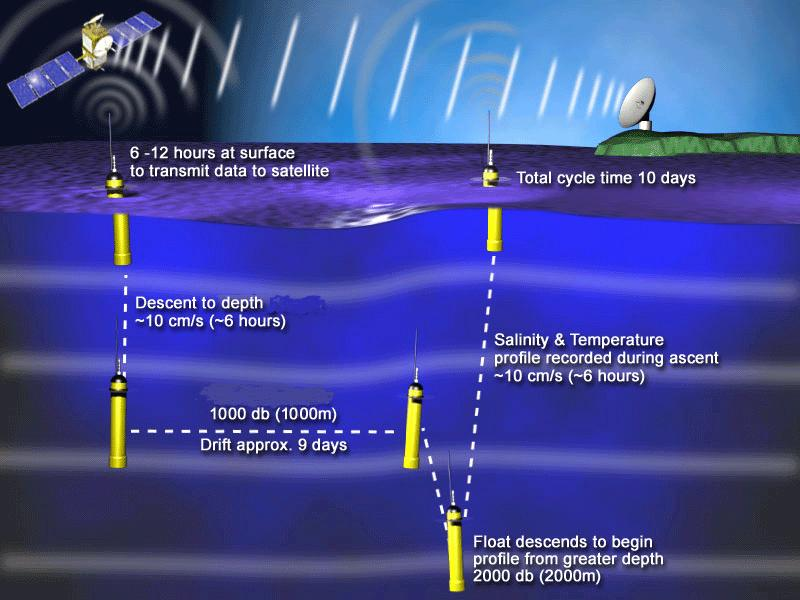
\includegraphics{pix/operation_park_profile.jpg}
        \caption[Argos Messzyklus - Bildquelle: http://www.argo.ucsd.edu]{Argos  Messzyklus}
        \label{fig:Argo-messzyklus}
    \end{figure}

    Die Argo Treibbojen werden mit Schiffen an spezifischen Punkten ausgesetzt. Ein Messzyklus beträgt 10 Tage. Die Boje taucht am Anfang des Zyklus auf 1000 Meter Tiefe herab.  In dieser Tiefe verbringt die Sonde die nächsten 9 Tage. Anschließend sinkt sie auf die Maximale Tiefe von 2000 Metern herab um anschließend wieder zur Oberfläche aufzusteigen. An der Oberfläche sendet die Boje innerhalb von 6-12 Stunden die Daten über Iason an die Bodenstationen.
   
    \begin{figure}[!ht]
        \centering
        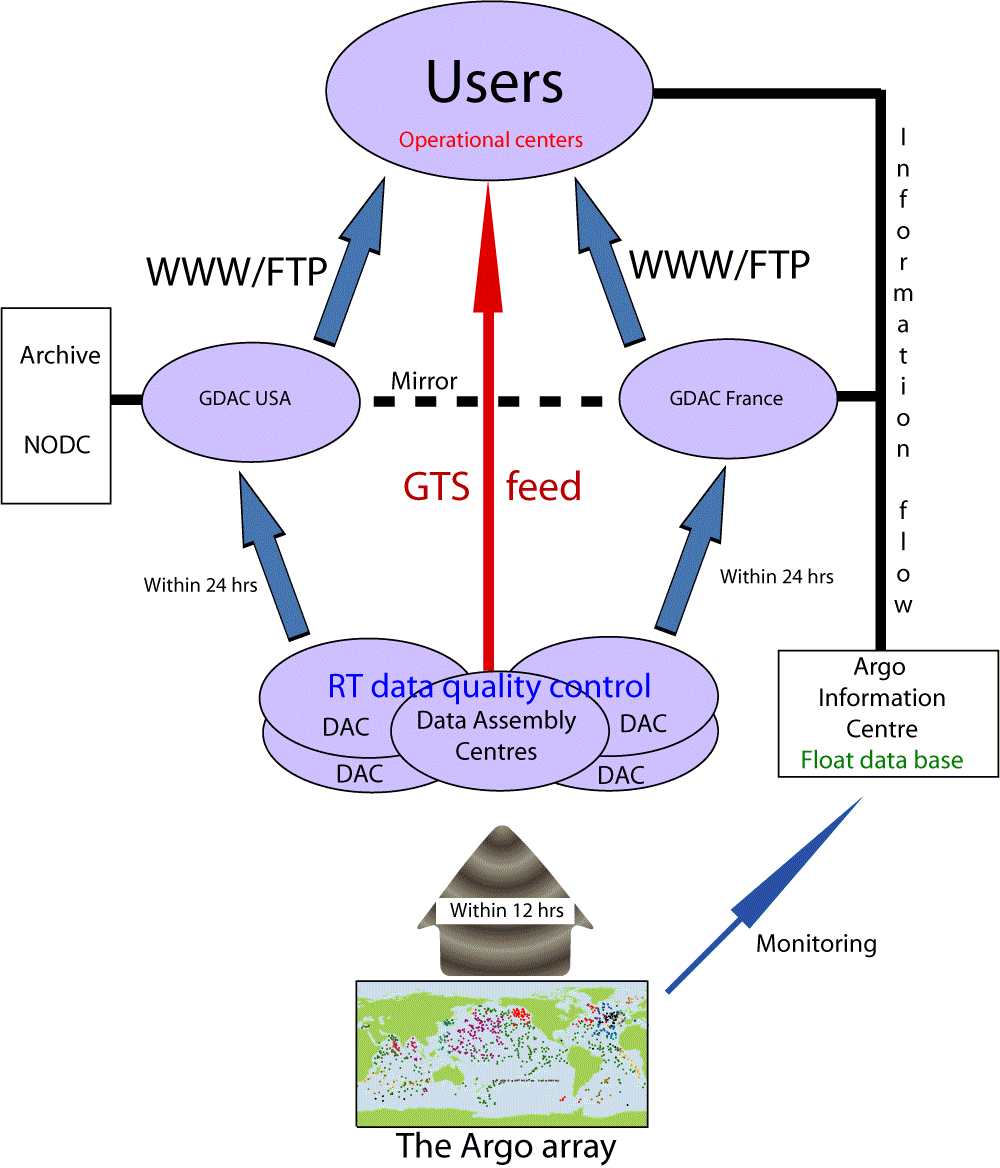
\includegraphics[width=0.4\textwidth]{pix/RT-Data-flow}
        \caption[Der Werdegang der Argo-Daten - Bildquelle: http://www.argo.ucsd.edu]{Der Werdegang der Argo-Daten}
        \label{fig:argo_dataflow}
    \end{figure}
    
    Nach der Erhebung werden die Daten auf deren Plausibilität und Qualität überprüft. \footnote{Siehe \cite{ArgoDataBeginnersGuide} Seite 3} Nach diesem Prozess werden die aufbereiteten Daten über die Globalen Data Assembly Center in monatlichen Releasezyklen veröffentlicht. \footnote{Siehe \cite{Argofloa92:online}}. Der Werdegang der Daten ist in Abbildung \ref{fig:argo_dataflow} zu sehen.

% BEGIN -- Daten
\subsubsection{Daten des Argo Programmes}
    

    Alle am Argo teilnehmenden Organisationen verpflichten sich auf eine gemeinsame Datenpolitik. So gibt es keine Herrschaft über die erhobenen Daten. Vielmehr stehen diese ab dem Zeitpunkt der Veröffentlichung transparent der Öffentlichkeit zur Verfügung.
    
    Nachdem die Daten von Iason aus dem Argo Array an die Data Assembly Centers übermittelt hat, werden diese einer Qualitätskontrolle unterzogen. Die Daten werden auf Plausibilität und Abweichungen überprüft. Nach dieser Qualitätskontrolle werden die Daten nun über die Global Data Assembly Centers in Frankreich und den USA released. Diese können dann über HTTP und FTP abgerufen werden. 
    
    Ein mal Im Monat werden die daten als Snapshots, den sogenannten DOI (digital object identifier) released. 
% END
    
% BEGIN -- Datenformate
\subsubsection{Datenformate}
    
    Während und vor der Qualitätskontrolle liegen die Daten im TESAC und BUFR Format vor. 
    
    Die von den DGACs veröffentlichten Daten stehen dann im Format NetCDF vor. Diese sind unter der Lizenz Attribution 4.0 International (CC BY 4.0) veröffentlicht und dürfen unter der Nennung der Lizenz frei verwendet und dabei auch verändert werden.
    
    \cite{ArgoDataDocumentation}
% END
    
% BEGIN -- Datenstruktur
\subsubsection{Datenstruktur}

In Listing \ref{lst:dataOrdnerstruktur} ist die Ordner Struktur der netCDF Dateien zu erkennen. Über den Ordnernamen aoml ist die Herkunft des DOI zu erkennen. In diesem Fall wurden die Dateien von einem Server der  Atlantic Oceanografic \& meterolocical Laboratory erstellt. Hier befindet sich für jede Messboje ein Unterordner. In diesem Fall sind die Ordner der Bojen 1900200 und 1900201 zu sehen. Die Dateien meta, prof, Rtraj und tech sind eine Quelle für Metainformationen. (TODO Was steht in den metadaten?) Die Messprofile einer Boje finden sich im Ordner \texttt{profiles}. Hier wird für jeden messzyklus eine Datei angelegt. Dieser startet bei 1 und inkrementiert über jeden Messzyklus um 1.
    
    \begin{python}[label={lst:dataOrdnerstruktur}, caption={test}]
./aoml/1900200/
- 1900200_meta.nc
- 1900200_prof.nc
- 1900200_Rtraj.nc
- 1900200_tech.nc
- profiles
    - D1900200_001.nc
    ...
    - D1900200_215.nc
    - D1900200_216.nc
./aoml/1900201/
...\end{python}

% END
    
